% !TEX root = ../my-thesis.tex
%
\chapter{Metodología}
\label{sec:methodology}


%\begin{figure}[htb]
%	
\includegraphics[width=\textwidth]{gfx/Clean-Thesis-Figure}
%	\caption{Figure example: \textit{(a)} example part one, \textit{(c)} example part two; \textit{(c)} example part three}
%	\label{fig:system:example1}
%\end{figure}

En esta sección revisamos el método propuesto para probar nuestra hipótesis junto a las consideraciones tomadas para su uso. Las divisiones principales se enfocan en: la preparación del modelo geométrico utilizado para la aproximación estructural y las propiedades bioelectromagnéticas de los tejidos incluidas las variaciones de conductividad, la solución del problema directo utilizando dipolos eléctricos que modelan puntos fijos de actividad neuronal equivalentes a respuestas evocadas (ER por sus siglas en inglés\footnote{Evoked response}) y un vector tridimensional de magnitud variable que representa el comportamiento de dicho dipolo, la solución del problema inverso de las señales simuladas para identificar la posición de las fuentes de actividad neuronal, y por último un análisis estadístico del estimador utilizando la frontera de Cramer-Rao para verificar su desempeño como estimador no sesgado.

\section{Método Propuesto}
\label{sec:methodology:method}

%Introduce your overall approach

Con la finalidad de estimar el BSCR, diseñamos un experimento que nos permitiría construir un estimador al implementar una solución del problema inverso con datos completamente simulados, y por ende con total control sobre las variables definidas como: la conductividad, la posición, orientación y magnitud de las fuentes de actividad neuronal, y el ruido añadido a las mediciones. El proceso del experimento es una implementación completa del problema directo e inverso del EEG con un posterior análisis estadístico, el problema directo nos permite obtener un modelo detallado de la actividad neuronal en la cabeza y simular mediciones de EEG con diferentes valores del BSCR, a su vez, el problema inverso resolverá las posiciones de las fuentes simuladas utilizando las mediciones generadas por el modelo del problema directo, y el análisis estadístico nos permitirá obtener la estimación de los valores de conductividad con base en el error incurrido en la localización de las fuentes de actividad neuronal respecto a su posición real agrupando por los distintos valores de conductividad utilizados. Basándonos en trabajo previo, decidimos implementar un método de la solución del problema inverso utilizando filtros espaciales (\emph{beamforming}) el cual es catalogado como un método paramétrico, también conocido como Método de Dipolo de Corriente Equivalente \cite{Grech2008}. Como su nombre lo indica, estos métodos consisten en buscar en una serie predefinida de dipolos de corriente el que mejor se ajuste en su posición y orientación a las fuentes que generaron las mediciones de EEG. 

Con el fin de realizar esta prueba de ajuste de los dipolos de corriente equivalente (solución del problema inverso) es necesario obtener la solución del problema directo. Existen varios métodos para obtener dicha solución \cite{Mosher1999}, de los cuales elegimos el método de elementos de frontera (BEM) para modelos geométricamente realistas \cite{Ermer2001}. La razón de elegir este método radica en el precedente del uso de modelos con geometrías más sencillas en estudios similares \cite{Gutierrez2004}, esto debido a que el BEM resultaba ser no viable por su elevado gasto computacional al calcular de las matrices de ganancia. En la actualidad se cuenta con mayor facilidad de acceso a equipos de cómputo con el suficiente desempeño para obtener resultados en un tiempo razonable, esto aunado al desarrollo de métodos y software mucho más eficientes \cite{open,Clerc2010} nos presenta la posibilidad de implementar el BEM para geometrías realistas como una evolución natural de los métodos utilizados anteriormente.

\begin{figure}[htb]
	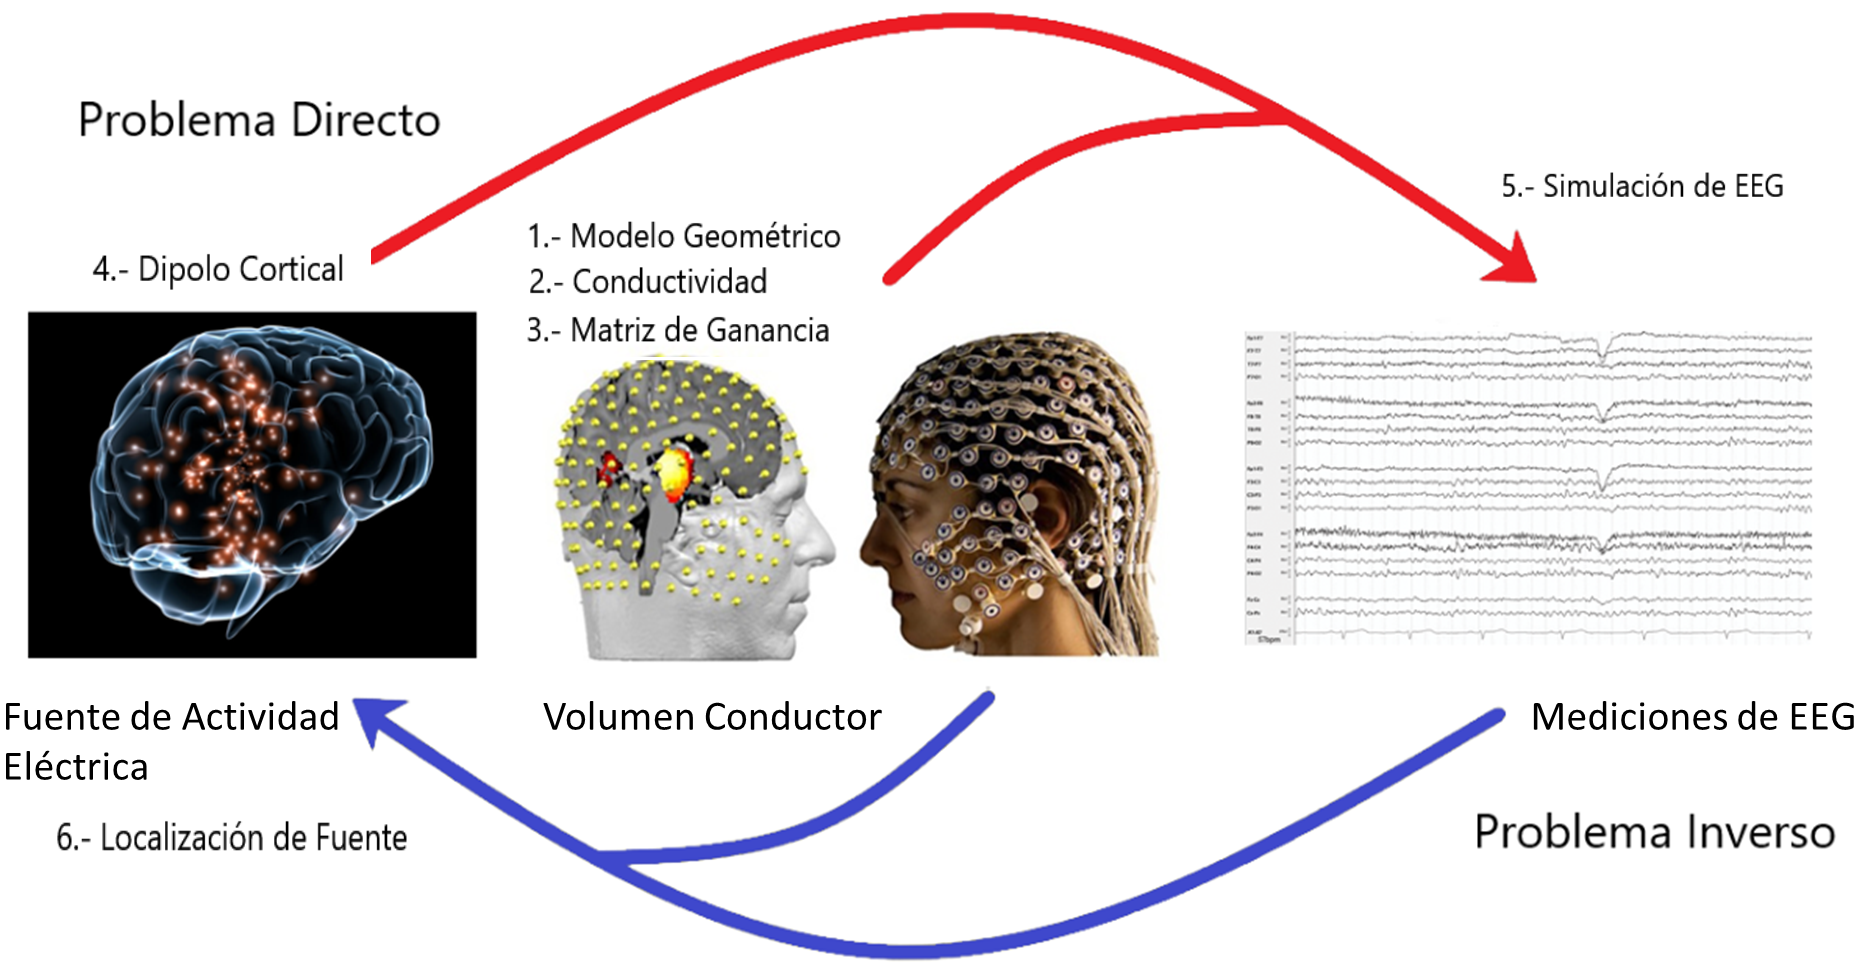
\includegraphics[width=\textwidth]{pipeline}
	\caption{Proceso del problema directo e inverso del EEG}
	\label{fig:methodology:pipeline}
\end{figure}


Una vez establecidos los métodos a utilizar en el método directo e inverso, se procedió a recopilar y formular la información necesaria para realizar los cálculos. En el caso del problema directo los datos de entrada requeridos son: el modelo geométricamente realista que representará a los tejidos de la cabeza como un volumen conductor, una serie de dipolos que modelan el fenómeno de respuesta evocada, los valores a probar de la conductividad entre los tejidos, en específico la razón cerebro/cráneo, y por último el arreglo de sensores de EEG que medirán el campo eléctrico simulado. Como resultado, se obtiene una matriz de ganancia dependiente de los valores de conductividad utilizados que dictamina como el arreglo de sensores de EEG captaría el campo eléctrico generado por las fuentes de actividad neuronal (dipolos) sobre la parte más superficial del modelo geométrico. Mientras que para el problema inverso, los datos de entrada consisten en: las mediciones de EEG simuladas a partir de la solución del problema directo, el mismo modelo geométrico con su arreglo de EEG correspondiente, las matrices de ganancia generadas en el problema directo, y las propiedades pertinentes al método de beamforming, como la matriz de covarianza de las mediciones y una matriz de covarianza del ruido. Como resultado final de este método, obtenemos un kernel de proyección de las fuentes de actividad neuronal que el beamformer pudo localizar. Lo que nos permite comparar la posición de los dipolos que fueron fijados en un principio en el problema directo contra la posición localizada por el beamformer con respecto a los diferentes valores de conductividad, y así obtener un estimador basado en los errores incurridos en la localización de estas fuentes. 


\section{Construcción del Modelo Geométricamente Realista}
\label{sec:methodology:model}


\begin{figure}[htb]
	\centering
	\begin{subfigure}{0.49\textwidth}
		\centering
		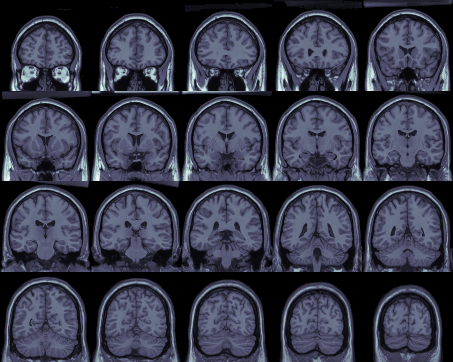
\includegraphics[width=\textwidth]{mri_coronal}
		\caption{Corte coronal}
		\label{fig:left}
	\end{subfigure}
	\begin{subfigure}{0.49\textwidth}
		\centering
		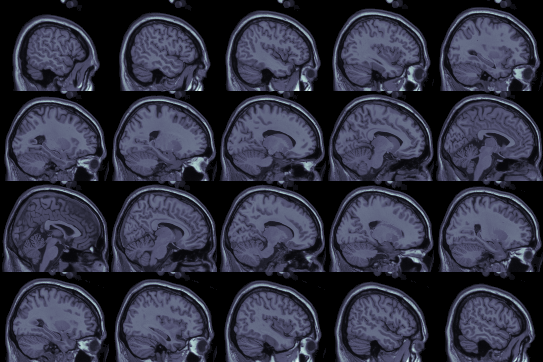
\includegraphics[width=\textwidth]{mri_sagital}
		\caption{Corte sagital}
		\label{fig:top_right}
	\end{subfigure}
	\begin{subfigure}{0.49\textwidth}
		\centering
		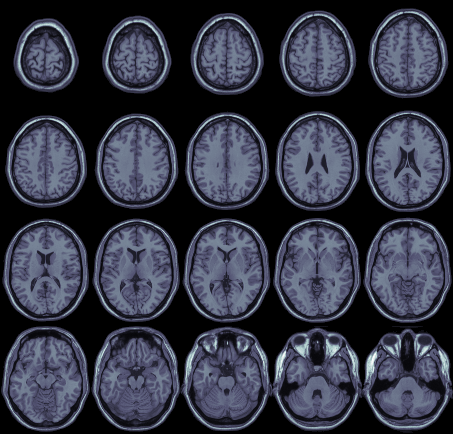
\includegraphics[width=\textwidth]{mri_axial}
		\caption{Corte axial} % You can change the caption here
		\label{fig:bottom_right} % You can change the label here
	\end{subfigure}
	\caption{Resonancia magnética de Colin27}
	\label{fig:combined}
\end{figure}


Entrando en detalles, la construcción del modelo geométricamente realista de los tejidos se basó en la plantilla ``Colin27 Average Brain 2008'' realizada por Aubert-Broche \emph{et al} \cite{Aubert-Broche2006}. Esta consiste en una versión mejorada del modelo de Colin que resulta del promedio de 27 imágenes de resonancia magnética ponderadas en T1, T2, y densidad protónica, provenientes de diferentes mediciones del mismo sujeto \cite{Holmes1998}. 

Con la información recopilada de la anatomía del sujeto se generó mediante el software libre Brainstorm\cite{brain2011} un conjunto de mallas teseladas y anidadas que representan las fases entre los diferentes tejidos de interés \emph{i.e.} cerebro, cráneo, y cuero cabelludo. Dado el alto costo computacional la resolución de las mallas es diferente dependiendo de la profundidad de las fases, siendo cerebro/cráneo y cráneo/cuero cabelludo (\cref{fig:methodology:inner,fig:methodology:outer}) las que mayor resolución tienen; 8640 triángulos y 4322 vértices, debido a que estas tienen una mayor sensibilidad al ser las más cercanas a la fuente de actividad neuronal y que representan por completo la capa de tejido óseo que servirá como volumen conductor, por estas razones es importante que ambas mallas tengan la misma resolución y no comprometan la precisión de los resultados. La fase del cuero cabelludo/aire (\cref{fig:methodology:head}) tiene una resolución menor con 6480 triángulos y 3242 vértices, esta fue definida así porque fue el límite de resolución computable con la RAM de la workstation, aún así, esta es una resolución alta comparada con el uso recomendado del software \cite{Tadel2019}. Por último se tiene una malla que representa la corteza cerebral (\cref{fig:methodology:cortex}), esta tiene una resolución de 29988 triángulos compuestos de 15002 vértices, los cuales son importantes mencionar porque la finalidad de esta malla es tener un arreglo de ``dipolos elementales'' sobre los que se proyectarán los resultados, por esta razón aunque la malla es importante para el cálculo del campo eléctrico generado por actividad neuronal no influye drásticamente en el costo computacional y puede utilizarse una resolución mayor para representar con detalle los pliegues y concavidades de la corteza cerebral. Todas las mallas en conjunto representan nuestro volumen conductor (\cref{fig:methodology:model}) sobre el que se implementarán los cálculos de BEM y la proyección del resultado del beamformer.

\begin{figure}[htb]
	\centering
	\begin{subfigure}{0.45\textwidth}
		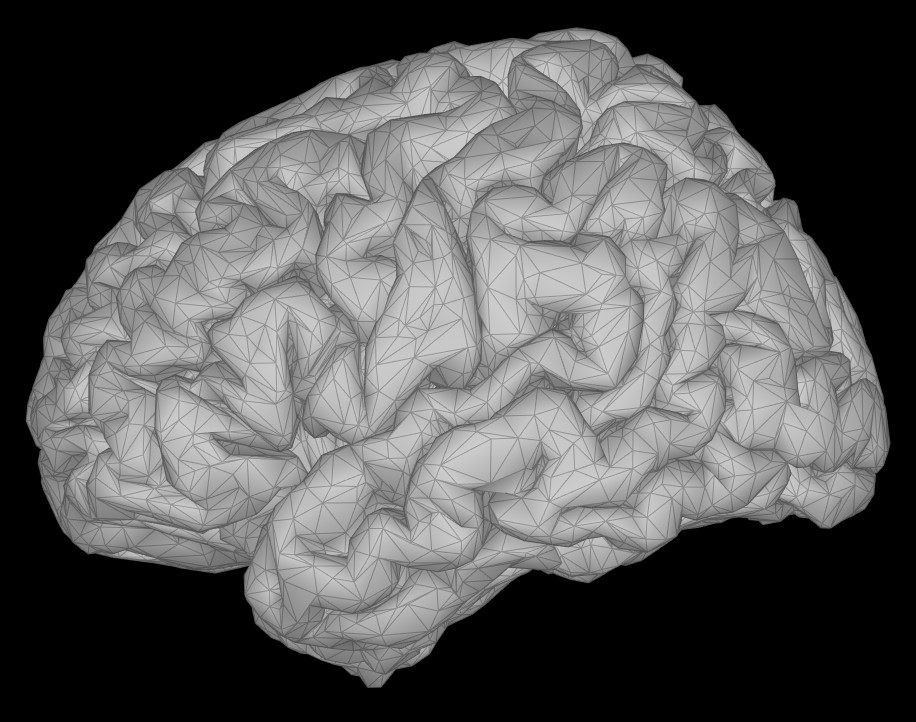
\includegraphics[width=\textwidth]{cortex}
		\caption{Corteza cerebral}
		\label{fig:methodology:cortex}
	\end{subfigure}\hfill
	\begin{subfigure}{0.45\textwidth}
		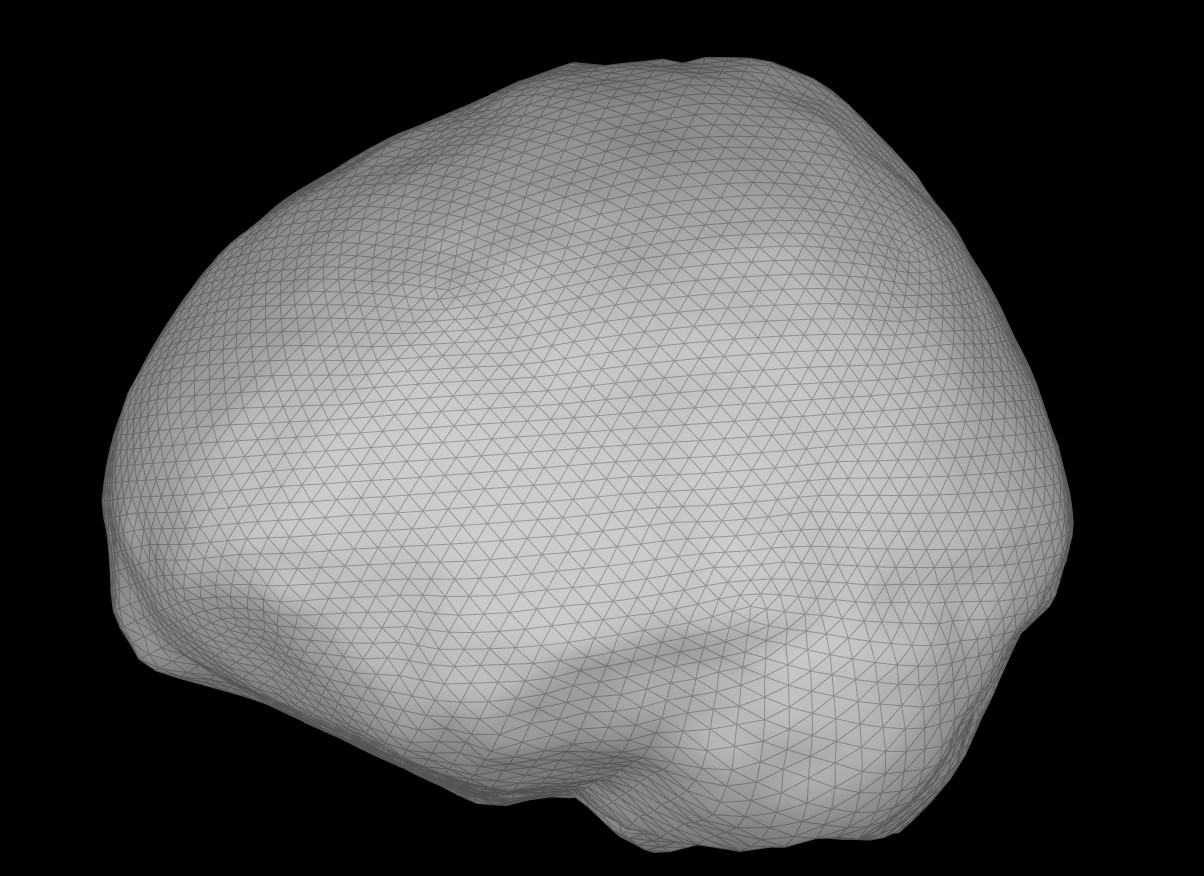
\includegraphics[width=\textwidth]{inner}
		\caption{Capa interna del cráneo}
		\label{fig:methodology:inner}
	\end{subfigure}\\
	\begin{subfigure}{0.45\textwidth}
		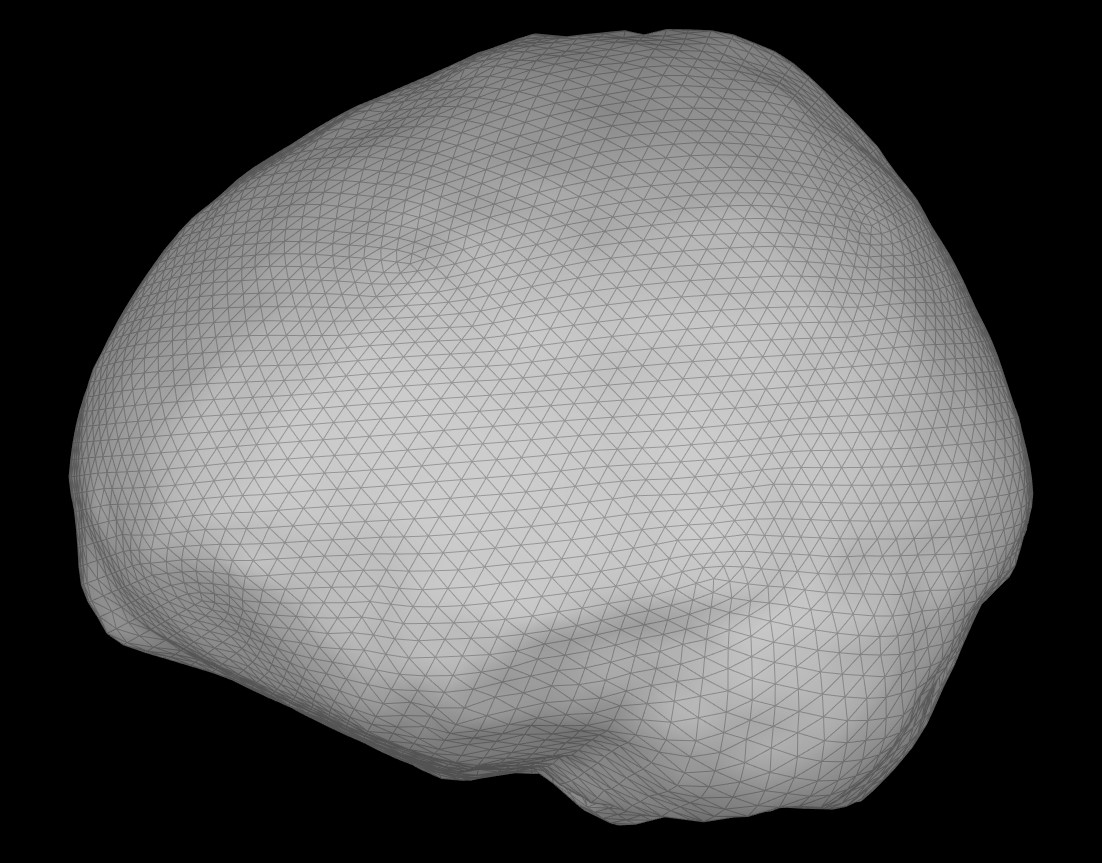
\includegraphics[width=\textwidth]{outer}
		\caption{Capa externa del cráneo}
		\label{fig:methodology:outer}
	\end{subfigure}\hfill
	\begin{subfigure}{0.45\textwidth}
		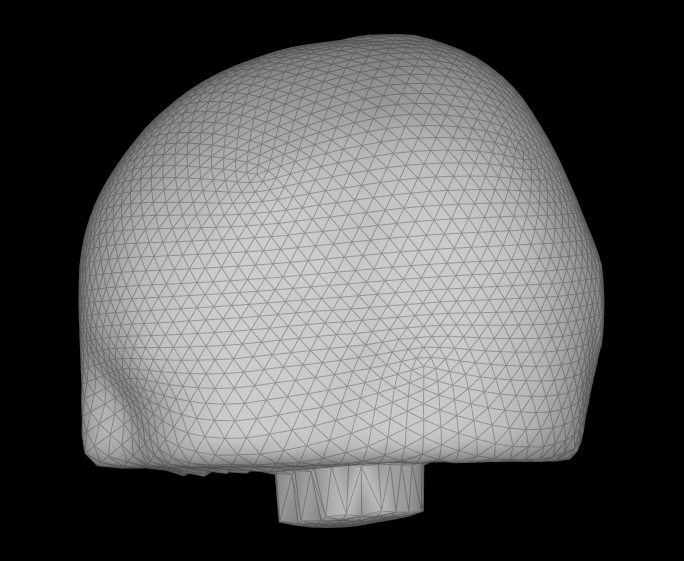
\includegraphics[width=\textwidth]{head}
		\caption{Cuero cabelludo}
		\label{fig:methodology:head}
	\end{subfigure}
	\caption{Mallas de las diferentes fases de los tejidos de la cabeza}
	\label{fig:methodology:meshes}
\end{figure}



\begin{figure}[htb]
	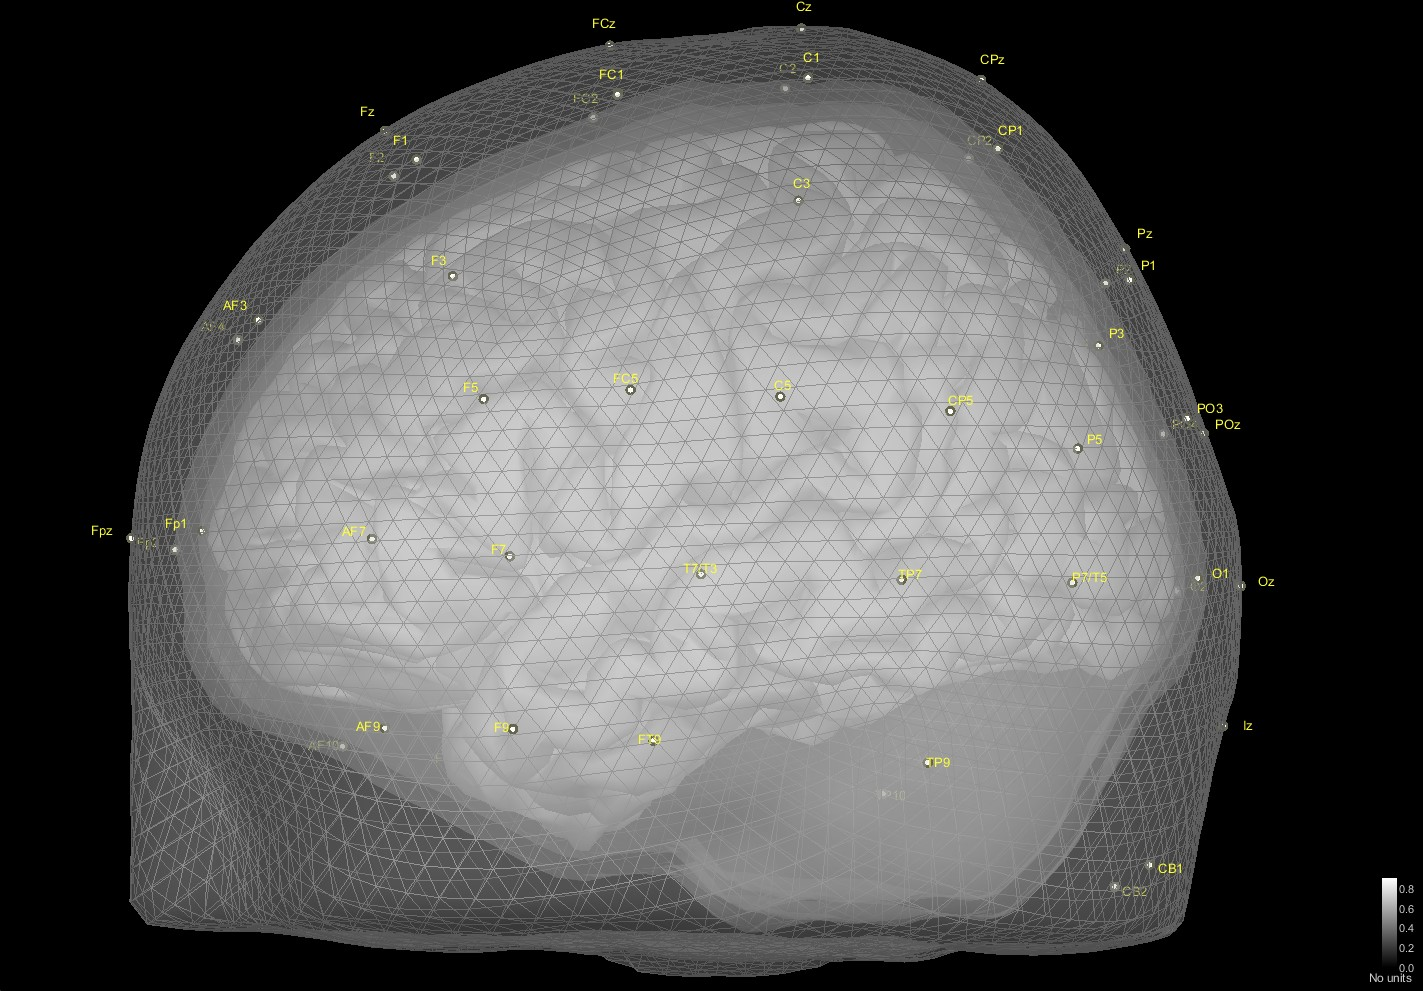
\includegraphics[width=\textwidth]{modelo}
	\caption{Modelo geométricamente realista}
	\label{fig:methodology:model}
\end{figure}




\section{Variación de la conductividad y cálculo de la matriz de ganancia por el método de elementos de frontera}
\label{sec:methodology:openmeeg}

Recapitulando, lo necesario para la solución del problema directo es: una fuente de corriente eléctrica y un modelo de un volumen conductor con la conductividad de los tejidos que representan. Usualmente, la finalidad de la implementación del problema directo es ubicar la posición de la fuente de corriente que representa la actividad neuronal por lo que esta ubicación es la variable independiente al momento de hacer el cálculo, mientras que la conductividad se mantiene como un valor fijo. 

En el área de neurociencias se suele mantener un valor estandarizado para la razón de conductividad cerebro-cráneo de 1:80 (\emph{i.e.} $0.33\text{ S/m}$ para el cerebro y $0.0042 \text{ S/m}$ para el cráneo) \cite{Rush1968,Rush1969,Cohen1983}. Sin embargo, múltiples estudios con diferentes acercamientos han publicado valores de la razón de conductividiad cerebro-cráneo (BSCR por sus siglas en inglés\footnote{Brain-scalp-conductivity-ratio}) que se desvían significativamente del estandár de 1:80 \cite{McCann2019}. Razón por la cual el objetivo de nuestro experimento es estimar el valor del BSCR al utilizarlo como la variable independiente mientras se toma por conocida la posición del dipolo de corriente además de mantenerse fija para todos los experimentos.

Regresando a la \cref{lineal} $B$ representa la llamada \emph{matriz de ganancia} que determina la sensibilidad del arreglo de electrodos en un EEG y como estos registrarán el campo eléctrico sobre el cuero cabelludo. Para el cálculo de esta matriz de ganancia por medio de BEM se utilizó el software OpenMEEG \cite{open,open2}, donde se utilizaron como datos de entrada nuestro modelo geométricamente realista, un arreglo de EEG de 10-10 (65) IMAGEN DEL ARREGLO, y los valores de conductividad del cerebro, cráneo, y cuero cabelludo. Se completó el cálculo de la matriz de ganancia para 10 TABLA DE CONDUCTIVIDADES valores del BSCR de los cuales 2 son valores aceptados en la literatura (1:20, 1:80) y los 8 restantes se eligieron de una revisión realizada por McCann \cite{McCann2019}, el criterio para la elección de estos 8 fue el hecho que su estimación se realizó con métodos que involucraban el uso de EEG, EEG/MEG, esto con el fin de mantener relación con nuestra propia estimación y compararlos objetivamente. La matriz resultante de cada una de los valores del BSCR tiene forma de (45006 X 65), que corresponden a los 65 canales del EEG y su respuesta a los 15002 vértices de la malla de la corteza cerebral del modelo geométrico en sus tres componentes vectoriales.

\section{Dipolos de corriente e implementación de la solución del problema directo}
\label{sec:methodology:direct_solved}

La matriz de ganancia de cada BSCR con el modelo geométrico completan el volumen conductor con sus propiedades electromagnéticas, la pieza restante para el cálculo del problema directo es la fuente de actividad eléctrica que se propagará por dicho volumen conductor. Como se había discutido anteriormente se decidió usar un dipolo eléctrico de posición fija gracias a que la actividad neuronal correspondiente a un ER se puede modelar como tal, este dipolo varía su magnitud con el tiempo en un periodo de 600 ms FIGURA DEL DIPOLO. En cuanto a la posición, se decidió utilizar tres diferentes, cada una en distintas zonas del cerebro correspondientes a lugares de eventos de respuesta evocada, siendo estas: la corteza somatosensorial primaria (coordenadas MNI -52.2, -32.4, 55.8), corteza visual primaria (9.7, -98.6, 2.4), y corteza auditiva primaria (-65.0, -24.7, 11). Cabe mencionar que el sistema de coordenadas MNI ( CITAR http://www.bic.mni.mcgill.ca/~louis/stx\_history.html) es usualmente utilizado como referencia para la comparación de diferentes sujetos, pero el software utiliza para sus cálculos el sistema CTF/MRI al que denomina \emph{Subject Coordinate System} (SCS), por lo que toda futura mención de coordenadas corresponden a dicho sistema.

Teniendo satisfechos los requisitos para la solución del problema directo este se calculó de la siguiente forma: dentro del software Brainstorm se crearon \emph{scouts} en la malla de la corteza cerebral que consisten en las coordenadas SCS de las regiones de interés (ROI\footnote{Region-of-interest})estos fueron llamados \emph{dip1} (somatosensorial), \emph{dip2} (visual), y \emph{dip3} (auditiva), los scouts fueron utilizados como dato entrada junto con la función del dipolo con respecto al tiempo, el volumen conductor compuesto por el modelo geométricamente realista y la matriz de ganancia de cada BSCR, y por último el arreglo de sensores de EEG. Como resultado obtuvimos 10 mediciones de EEG simuladas correspondientes a cada BSCR para cada uno de los tres scouts, siendo en total 30 mediciones de EEG. Tomando en cuenta de que estamos simulando nuestros datos y estamos en control de todas las variables, se procedió a añadir ruido en la implementación del problema directo para considerar otras condiciones de experimentos con pacientes, el ruido se añadió con una relación señal/ruido (SNR\footnote{Signal-to-noise-ratio}) de $0.01\text{, } 0.05\text{, } \text{y } 0.1$. Obteniendo así 3 sets de 10 mediciones para cada uno de los 3 dipolos, resultando en 90 mediciones de EEG diferentes.


\section{Problema Inverso del EEG}
\label{sec:system:inverse}

Como su nombre lo indica; la contraparte del problema directo del EEG es el problema inverso. Si el problema directo se enfoca en obtener una solución para el campo eléctrico generado sobre un volumen conductor a partir de una fuente de corriente, el problema inverso consiste en identificar la posición de dichas fuentes de actividad eléctrica al modelar la amplitud de los dipolos eléctricos y seleccionando los que tengan una mayor actividad \cite{Baillet2001}. Para su cálculo es necesario: las mediciones de EEG que en nuestro caso son las obtenidas mediante el problema directo, el volumen conductor, ya la matriz de ganancia con su correspondiente mapa del sistema de EEG.

Dado que nuestro objetivo es la estimación del BSCR la forma en la que se implementó el problema inverso para la construcción de nuestro estimador fue la siguiente: Para cada uno de los 3 dipolos y su nivel de ruido correspondiente, se acomodaron los resultados del problema directo pareados con la matriz de ganancia de cada BSCR a probar, dando un total de 900 combinaciones diferentes. Con el fin de aumentar la robustez del estimador y evitar un sesgo, se realizaron 100 implementaciones del problema inverso por cada una de esas 900 combinaciones, obteniendo en total 900,000 mapas del índice de actividad neuronal (NAI\footnote{Neural activity index}) sobre la corteza cerebral que corresponden a las soluciones del problema inverso.

\section{Implementación del Problema Inverso del EEG}

Al igual que en la implementación del problema directo se uso en parte el software Brainstorm en Matlab, específicamente las librerías pertinentes para el procesado de las mediciones de EEG, estas fueron extraídas y modificadas para manejar de forma óptima el procesamiento de nuestro gran volumen de información. Como se mencionó anteriormente, el problema inverso da como resultado un mapa del índice de actividad neuronal sobre el volumen geométricamente realista, detallando como se propaga el campo eléctrico desde su origen en la corteza cerebral, hasta la superficie de la capa más externa, pasando por las fases internas FIGURA IMAGING KERNEL THROUGHOUT LAYERS. Para la solución del problema inverso se eligió el método de filtrado espacial \emph{Beamforming} linealmente constreñido de varianza mínima (LCMV\footnote{Linearly constrained minimum variance beamforming}) diseñado por VanVeen y Buckley\cite{VanVeen1988}, la implementación de este filtro que se incluye en Brainstorm produce mapas del pseudo índice de actividad neuronal (PNAI) llamado así por las modificaciones realizadas por Mosher \emph{et al.}\cite{Jaiswal2020} al Beamformer de VanVeen.

Este método de procesado digital de señales filtra...






\section{Frontera de Cramer-Rao}
\label{sec:system:conclusion}



